\documentclass[tikz,border=10pt]{standalone}
% Coordinates in cm, origin at O, scale s = 0.014953 cm per px, y flipped
\begin{document}
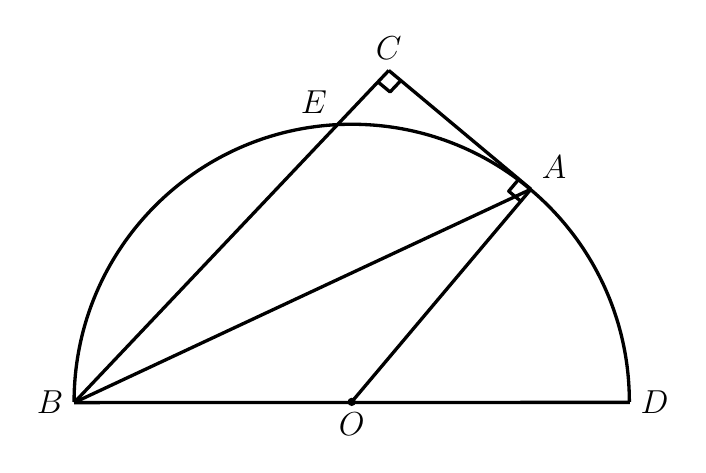
\begin{tikzpicture}[line width=1.2pt, line join=round]
  % Named points
  \coordinate (O) at (0,0);
  \coordinate (B) at (-3.525,-0.009);
  \coordinate (D) at (3.531,-0.006);
  \coordinate (A) at (2.276,2.701);
  \coordinate (C) at (0.471,4.209);
  \coordinate (E) at (-0.178,3.528);

  % Diameter BD and upper semicircle (arc, not full circle)
  \draw (B) -- (D);
  \draw (-3.526,0) arc[start angle=180, end angle=0, radius=3.526];

  % Triangle and segment AO
  \draw (B) -- (C);
  \draw (C) -- (A);
  \draw (A) -- (B);
  \draw (A) -- (O);

  % Right angle at C (between CB and CA)
  \draw (0.333,4.064) -- (0.487,3.936) -- (0.624,4.081);

  % Right angle at A (between AO and AC)
  \draw (2.147,2.548) -- (1.994,2.676) -- (2.123,2.829);

  % Filled dot at centre O, drawn after all strokes so it sits on top
  \fill (O) circle (1.5pt);

  % Labels with requested font
  \node[above] at (C) {\fontsize{12.5}{15}\selectfont $C$};
  \node[above left] at (E) {\fontsize{12.5}{15}\selectfont $E$};
  \node[above right] at (A) {\fontsize{12.5}{15}\selectfont $A$};
  \node[left] at (B) {\fontsize{12.5}{15}\selectfont $B$};
  \node[right] at (D) {\fontsize{12.5}{15}\selectfont $D$};
  \node[below] at (O) {\fontsize{12.5}{15}\selectfont $O$};
\end{tikzpicture}
\end{document}